\section{Ausgangslage}

Als Grundlage wird das Sprachdesign von IML dienen, wie es zur Verfügung gestellt wurde. In einer ersten 
Phase wurde ein Compiler für diesen Sprachumfang entwickelt, welcher danach für die in diesem Dokument
beschriebenen Erweiterungen angepasst wurde. Dieser Compiler wurde auf Basis der Sprache Scala entwickelt,
da diese einerseits funktionale Aspekte beim Programmieren ermöglicht, andererseits bereits 
Parser-Kombinatoren im Sprachumfang enthalten sind.


\newpage

%\begin{figure*}[h]
%	\begin{center}
%		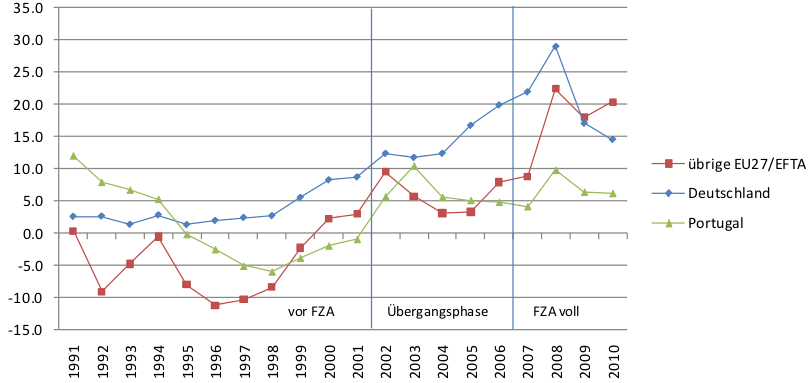
\includegraphics[width=0.9\textwidth]{images/Zuwanderungssaldo_Bericht_2.png}
%	\end{center}
%	\caption{Verlauf der Zuwanderung nach Herkunftsländern in Tausend \cite[S. 18]{ADMIN:Bericht}}
%	\label{fig:zuwanderungsaldi}
%\end{figure*}

